\documentclass[12pt]{article}

\usepackage[margin = .8in]{geometry}
\usepackage{amsmath}
\usepackage{graphicx}
\usepackage{multicol, enumerate, tabularx}

\usepackage{adjustbox}

\usepackage{fancyhdr}
\pagestyle{fancy}

\lhead{Math F113X: Numbers and Society}
\rhead{Date: \hspace{1in}}

\usepackage{tikz}
\usetikzlibrary{calc,trees,positioning,arrows,fit,shapes,through, backgrounds}
\usetikzlibrary{patterns}

\usetikzlibrary{decorations.markings}
\usetikzlibrary{arrows}

\usepackage{pgfplots}

\usepackage{longtable}
\usepackage{tabularx}

\newcommand{\ds}{\displaystyle}
\newcommand{\ans}[1][1in]{\rule{#1}{.5pt}}

\newcommand{\points}[1]{(#1 points.)}		% Trying to be lazy.

\usepackage{array}
\newcolumntype{L}[1]{>{\raggedright\let\newline\\\arraybackslash\hspace{0pt}}m{#1}}
\newcolumntype{C}[1]{>{\centering\let\newline\\\arraybackslash\hspace{0pt}}m{#1}}
\newcolumntype{R}[1]{>{\raggedleft\let\newline\\\arraybackslash\hspace{0pt}}m{#1}}
\newcommand{\red}[1]{\textcolor{red}{#1}}

\newcommand{\be}{\begin{enumerate}}
\newcommand{\ee}{\end{enumerate}}

%\topmargin -1in
%\textheight 9.5in
%\oddsidemargin -0.3in
%\evensidemargin \oddsidemargin
%\pagestyle{empty}
%%\marginparwidth 0.5in
%\textwidth 7in
%\parindent 0in

%--------------------------------------------------------------------------------------------------------------------------------------------------------------------------
%						Document
%--------------------------------------------------------------------------------------------------------------------------------------------------------------------------


\begin{document}
%\pagestyle{fancy}
\begin{center}
{\Large  Worksheet 13 (Graph Theory 5): Eulerization}
\end{center}



\noindent \textbf{Group Names:} \hrulefill \\
%-------------------------------------------------------------------------------------------------------------
%						Assignment
%-----------------------------------------------------------------------------------------------------
\begin{enumerate}

\item Consider the following graph.
\be
\item How many vertices of odd degree does this graph have? \ans 
\item Eulerize this graph: find the smallest number of edges you can add so that you can construct an {\bf Euler circuit}.
\item Draw the circuit on the graph.
\ee

\begin{center}

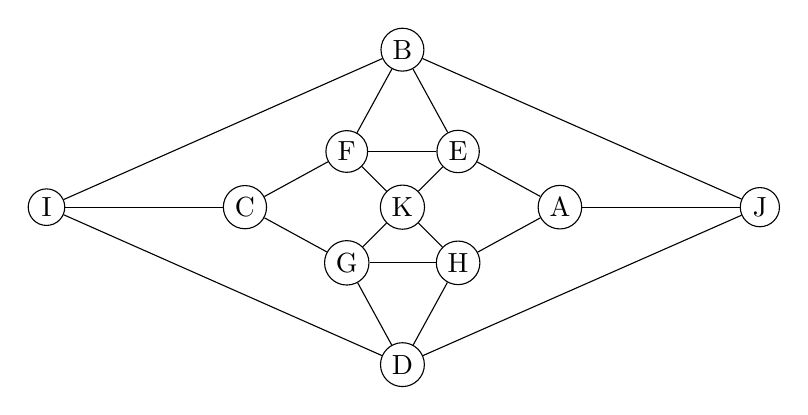
\begin{tikzpicture}[baseline=(current bounding box.center),]
\tikzstyle{vertex}=[circle, draw, inner sep=2pt]%, minimum size=6pt]

\tikzstyle{every node} = [vertex];
\node (A) at (0:2) {A};
\node (B) at (90:2) {B};
\node (C) at (180:2) {C};
\node (D) at (270:2) {D};
\node (O) at (0,0){K};
\node (E) at (45:1) {E};
\node (F) at (45+90:1){F};
\node (G) at (45+180:1){G};
\node (H) at (45+270:1){H};
\node[left  = 2 cm of C] (I) {I};
\node [right = 2 cm of A] (J) {J};
\draw (B) -- (I) -- (D) -- (J)--(B);
\draw (A) -- (E) -- (B) -- (F) -- (C) -- (G) -- (D) -- (H) -- (A);
\draw (E) -- (O) -- (G) (F) --(O) --(H);
\draw (A) -- (J) (C) -- (I);
%\draw (I) to[looseness = 3, distance = 2in] (J);
%\draw (I) to[looseness = 3, distance = -2in] (J);
\draw (E) -- (F)  (G) -- (H);
\end{tikzpicture}

\end{center}


\item Consider the following graph.
\be
\item Which are the vertices of odd degree? \hrulefill
\item Eulerize this graph: find the smallest number of edges you can add so that you can construct an {\bf Euler circuit}, and add them to the graph.
\item Draw the circuit on the graph.
\ee

\begin{center}
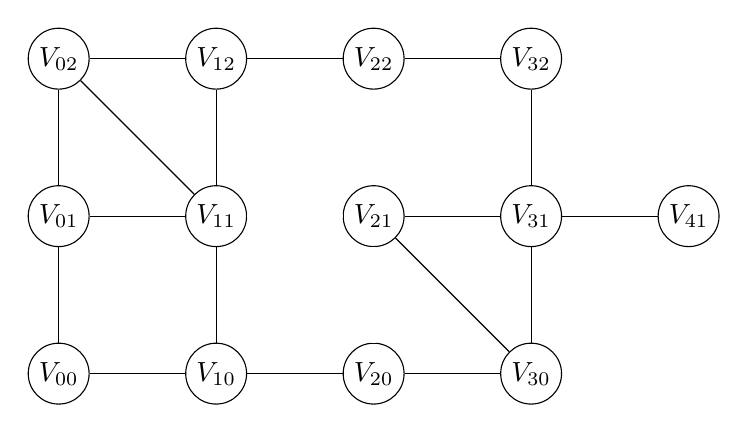
\begin{tikzpicture}[baseline=(current bounding box.center),]
\tikzstyle{vtx}=[circle, draw, inner sep=2pt]%, minimum size=6pt]
\foreach \i in {0,1,2,3}{
\foreach \j in {0,1,2}{
\node[vtx] (v\i\j) at (2*\i,2*\j){$V_{\i\j}$};
}}
\node[vtx] (v41) at (8,2){$V_{41}$};
\foreach \i in {0,1,2}{\foreach \j in {0,1,2} {\draw let \n1 = {int(\i+1)} in (v\i\j) -- (v\n1\j);}}
\foreach \i in {0,1,2,3}{\foreach \j in {0,1} {\draw let \n1 = {int(\j+1)} in (v\i\j) -- (v\i\n1);}}
\draw (v02) -- (v11);
\draw (v21) -- (v30);
\draw (v31)--(v41);
\draw[white, ultra thick] (v11)--(v21)(v22)--(v21)--(v20);
\end{tikzpicture}

\end{center}

\newpage

\item Consider the following weighted graph. 

\bigskip

\begin{center}

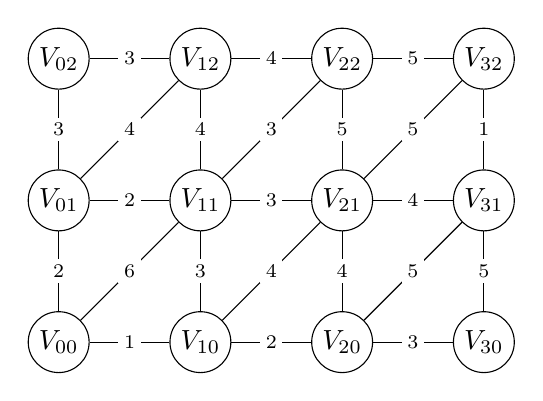
\begin{tikzpicture}[baseline=(current bounding box.center),lbl/.style={fill=white, inner sep = 2pt, font = \scriptsize}, scale = .9]
\tikzstyle{vtx}=[circle, draw, inner sep=2pt]%, minimum size=6pt]
\foreach \i in {0,1,2,3}{
\foreach \j in {0,1,2}{
\node[vtx] (v\i\j) at (2*\i,2*\j){$V_{\i\j}$};
}}
\foreach \i in {0,1,2}{\foreach \j in {0,1,2} {\draw let \n1 = {int(\i+1)}, \n2 = {int(\i+\j+1)} in (v\i\j) -- node[lbl]{\n2} (v\n1\j);}}
\foreach \i in {0,1,2,3}{\foreach \j in {0,1} {\draw let \n1 = {int(\j+1)}, \n2 = {int(\i+\j+2)} in (v\i\j) -- node[lbl]{\n2} (v\i\n1);}}
\draw (v22) --node[lbl]{3} (v11);
\draw (v21) --node[lbl]{4} (v10);
\draw (v12) --node[lbl]{4} (v01);
\draw (v32) -- node[lbl]{5} (v21);
\draw (v31) -- node[lbl]{5} (v20);
\draw (v11) -- node[lbl]{6} (v00);
\draw (v32) -- node[lbl]{1} (v31);

\end{tikzpicture}


\end{center}

\bigskip


\be
\item There are two vertices of odd degree in this graph, $V_{00}$ and $V_{32}$. Use Dijkstra's algorithm to find a path of minimum distance between the two vertices. Break ties by using the vertex whose subscript is smaller (for example, $V_{01}$ is smaller than $V_{23}$ because $01 = 1 < 23$.)

\vfill
\item Duplicate your minimum distance path (including the weights) to eulerize the graph.

\item Then find an Euler circuit in the graph of minimum total weight.

\begin{center}
\bigskip
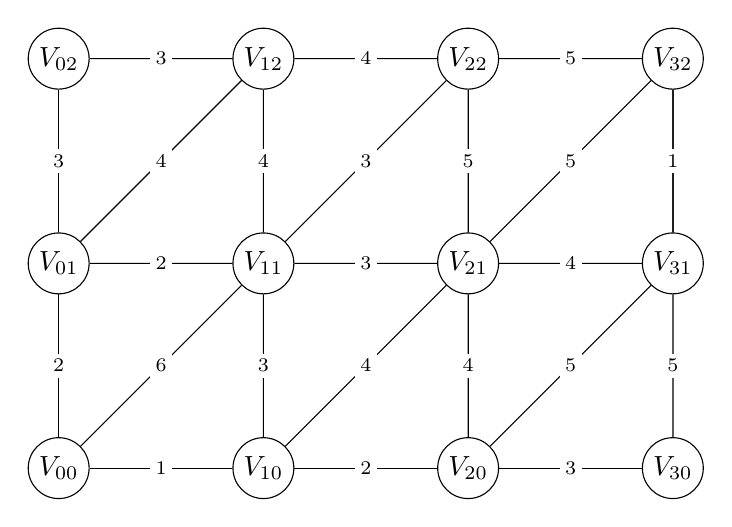
\begin{tikzpicture}[baseline=(current bounding box.center),lbl/.style={fill=white, inner sep = 2pt, font = \scriptsize}, scale  = 1.3]
\tikzstyle{vtx}=[circle, draw, inner sep=2pt]%, minimum size=6pt]
\foreach \i in {0,1,2,3}{
\foreach \j in {0,1,2}{
\node[vtx] (v\i\j) at (2*\i,2*\j){$V_{\i\j}$};
}}
\foreach \i in {0,1,2}{\foreach \j in {0,1,2} {\draw let \n1 = {int(\i+1)}, \n2 = {int(\i+\j+1)} in (v\i\j) -- node[lbl]{\n2} (v\n1\j);}}
\foreach \i in {0,1,2,3}{\foreach \j in {0,1} {\draw let \n1 = {int(\j+1)}, \n2 = {int(\i+\j+2)} in (v\i\j) -- node[lbl]{\n2} (v\i\n1);}}
\draw (v22) --node[lbl]{3} (v11);
\draw (v21) --node[lbl]{4} (v10);
\draw (v12) --node[lbl]{4} (v01);
\draw (v32) -- node[lbl]{5} (v21);
\draw (v31) -- node[lbl]{5} (v20);
\draw (v11) -- node[lbl]{6} (v00);
\draw (v32) -- node[lbl]{1} (v31);

\end{tikzpicture}

\end{center}

\ee

\end{enumerate}
\end{document}

%-------------------------------------------------------------------------------------------------------------------------------------------------------------------------------------------------------------------

%%% Local Variables:
%%% mode: latex
%%% TeX-master: t
%%% End:
